\bgroup
\begin{frame}{Blackjack Example}
\begin{minipage}{0.7\textwidth}
\begin{itemize}
\item States (200 of them):
\begin{itemize}
\item Current sum (12-21)
\item Dealer's showing card (ace-10)
\item Do I have a useable ace? (yes-no)
\end{itemize}
%
\item Action \textcolor{mImagelabRed}{stick}: Stop receiving cards (and terminate)
\item Action \textcolor{mImagelabRed}{twist}: Take another card (no replacement)
\item Reward for \textcolor{mImagelabRed}{stick}:
\begin{itemize}
\item +1 if sum of cards $>$ sum of dealer cards
\item 0 if sum of cards $=$ sum of dealer cards
\item -1 if sum of cards $<$ sum of dealer cards
\end{itemize}
%
\item Reward for \textcolor{mImagelabRed}{twist}:
\begin{itemize}
\item -1 if sum of cards $>$ 21 (and terminate)
\item 0 otherwise
\end{itemize}
%
\item Transitions: automatically \textcolor{mImagelabRed}{twist} if sum of cards $<$ 12
\end{itemize}
\end{minipage}
\begin{minipage}{0.25\textwidth}
\begin{figure}
\centering
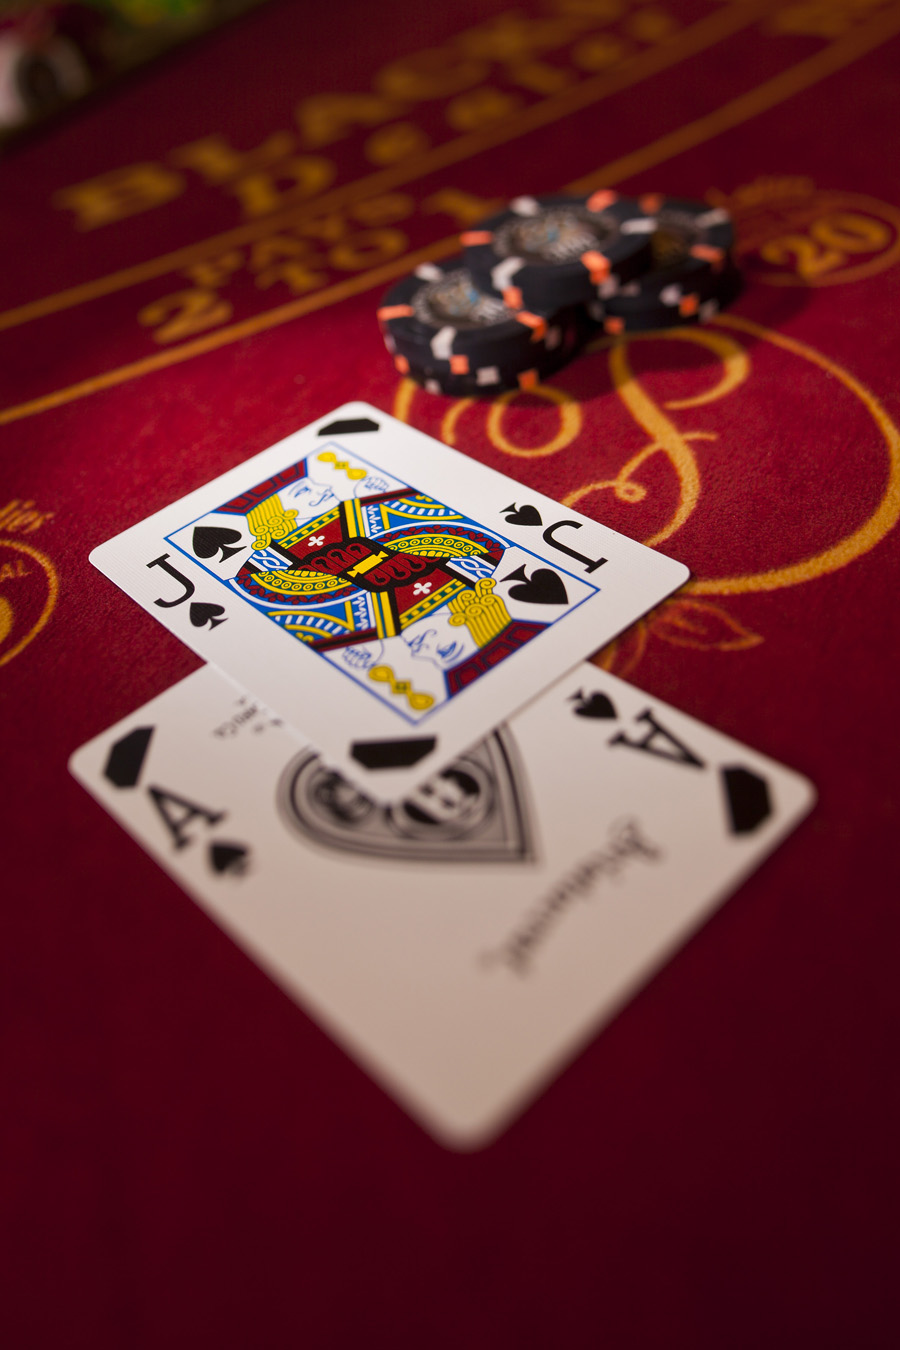
\includegraphics[width=\textwidth]{img/blackjack.jpg}
\end{figure}
\end{minipage}

\end{frame}
\egroup